% !TeX program = xelatex
% ============================================================
% 2026 年·北京卷数学（回忆版，内部候选） · 解析版
% 由 tools/make_editions.py 生成（重跑会覆盖本文件）；
% 题目/解析内容在 questions.tex / answers*.tex，勿在本文件内写内容。
% ============================================================
\documentclass[zihao=-4, a4paper]{ctexart}
% ============================================================
% common/preamble.tex —— 拆分版试卷项目 · 公共导言区
% 引擎：XeLaTeX；文档类 ctexart 由各版本壳文件自行声明
% 由合并书 math-gaokao-2017-2026/preamble.tex 改造而来：
%   - 页眉左右改为可重定义宏 \gkheadL / \gkheadR（各版本壳设置）
%   - hyperref 不再写死 pdftitle（壳内 \hypersetup 覆盖）
%   - 删除书籍专用的 \chaptermark 重定义与 \gkpaper 装配宏
% ============================================================

% ---------- 数学 ----------
\usepackage{amsmath}
\usepackage{amssymb}
\usepackage{mathtools}

% ---------- 绘图 ----------
\usepackage{tikz}
\usetikzlibrary{shapes.geometric, arrows.meta, calc, patterns, angles, quotes, positioning}
\usepackage{pgfplots}
\pgfplotsset{compat=1.18}

% ---------- 版面 ----------
\usepackage{geometry}
\usepackage{needspace}
\geometry{a4paper, margin=2.2cm, headheight=15pt}
% 紧凑版式（如印刷版）可在壳文件中于 \begin{document} 前再次调用 \geometry 覆盖
\usepackage{enumitem}
\setlist{itemsep=2pt, topsep=4pt, parsep=0pt}

% 中文与行内公式混排的断行弹性：
% emergencystretch 允许段落末路不通时追加伸展量；
% 降低二元/关系符罚分，允许行内长公式在 = 、+ 等处断行（否则整段外溢）
\emergencystretch=2em
\binoppenalty=700
\relpenalty=500
\usepackage{booktabs}      % 三线表
\usepackage[most]{tcolorbox}

% ---------- 选择题选项对齐 ----------
% tasks 宏包：\begin{gkopts}(列数) \task ... \end{gkopts}
% 自动等宽分栏，选项天然对齐；列数已由内容片段按选项长度写定（4/2/1）
\usepackage{tasks}
\settasks{label={}, label-width=0pt, item-indent=1.2em,
          column-sep=1em, after-item-skip=2pt, before-skip=2pt, after-skip=4pt}
\NewTasksEnvironment[style=itemize]{gkopts}[\task](4)

% ---------- 页眉页脚 ----------
\newcommand{\gkheadL}{}   % 左页眉：卷名（壳文件 \renewcommand 设置）
\newcommand{\gkheadR}{}   % 右页眉：版本名（壳文件 \renewcommand 设置）
\usepackage{fancyhdr}
\pagestyle{fancy}
\fancyhf{}
\fancyhead[L]{\small\gkheadL}
\fancyhead[R]{\small\gkheadR}
\fancyfoot[C]{\small —— 第 \thepage\ 页 ——}
\renewcommand{\headrulewidth}{0.4pt}

% ---------- 超链接（须最后加载）----------
\usepackage{hyperref}
\hypersetup{colorlinks=true, linkcolor=blue!55!black,
            bookmarksnumbered=true, unicode=true}

% ============================================================
% common/macros.tex —— 自定义命令与环境（题号、解析头、提示框等）
% 与合并书 math-gaokao-2017-2026/preamble.tex 的自定义段保持一致，
% 保证内容片段（questions.tex / answers.tex）在两个项目间可互换。
% ============================================================

% ---------- 试卷标识（壳文件 \renewcommand 设置，用于 label 命名空间）----------
\newcommand{\gkpaperid}{none}

% ---------- 题号 ----------
% 试题部分的题号：加粗编号 + 自动 \label{q:<卷id>:<题号>}
\newcommand{\gkti}[1]{\par\medskip\noindent
  \textbf{#1．}\phantomsection\label{q:\gkpaperid:#1}\ignorespaces}
% 多卷/分部重启题号时，#1 是唯一内部顺序号（交叉引用身份），#2 才是原卷显示题号。
\newcommand{\gktiwithlabel}[2]{\par\medskip\noindent
  \textbf{#2．}\phantomsection\label{q:\gkpaperid:#1}\ignorespaces}

% 解析部分的题头：小标题 + 回链到试题页
% （仅在题目与解析同文档的版本中回链有效；试题版不含解析头，无悬空引用）
\newcommand{\gksolhead}[2]{%
  \Needspace{3\baselineskip}\subsubsection*{第 #1 题\if\relax\detokenize{#2}\relax\else（#2）\fi}%
  \phantomsection\label{s:\gkpaperid:#1}%
  {\small\color{gray}（题目见第~\pageref{q:\gkpaperid:#1}~页）}\par\nopagebreak}
% 与 \gktiwithlabel 成对：显示原题号，但回链仍用唯一内部顺序号。
\newcommand{\gksolheadwithlabel}[3]{%
  \Needspace{3\baselineskip}\subsubsection*{第 #2 题\if\relax\detokenize{#3}\relax\else（#3）\fi}%
  \phantomsection\label{s:\gkpaperid:#1}%
  {\small\color{gray}（题目见第~\pageref{q:\gkpaperid:#1}~页）}\par\nopagebreak}

% ---------- 填空题空位 ----------
\newcommand{\gkblank}{\underline{\hspace{2.2em}}}

% ---------- 提示框 ----------
% 卷种提示 / 解析归属声明（醒目，浅黄）
\newtcolorbox{gknotice}{colback=yellow!8, colframe=orange!60!black,
  boxrule=0.5pt, arc=1.5pt, left=6pt, right=6pt, top=4pt, bottom=4pt,
  before skip=8pt, after skip=8pt}

% 方法提示 / 注（浅蓝，用于解析后的点评与题量说明）
\newtcolorbox{gktip}{colback=blue!4, colframe=blue!35!black,
  boxrule=0.4pt, arc=1.5pt, left=6pt, right=6pt, top=4pt, bottom=4pt,
  before skip=6pt, after skip=6pt, fontupper=\small}

% ---------- 答案行 ----------
% 解析中独立成段的"答案：X"用带底色的行呈现
\newcommand{\gkanswer}[1]{\par\smallskip\noindent
  \tcbox[width=\linewidth, tcbox width=auto limited,
         colback=green!6, colframe=green!35!black, boxrule=0.4pt,
         arc=1.5pt, left=4pt, right=4pt, top=2pt, bottom=2pt,
         nobeforeafter]{\textbf{#1}}\par\smallskip}

% ---------- 结构标题 ----------
% 结构标题后通常紧跟一个带 0.5\textheight 起始预留的解析题块；0.4 只够放标题，
% 会把下一题整体推到下一页，留下孤立的「二、填空题」等页尾标题。
\newcommand{\gkpart}[1]{\Needspace{0.6\textheight}\subsection*{#1}\nopagebreak}     % 标题 + 首题
% （一）必考题 / 解析小问标题：块式加粗段，可自动换行（\paragraph 的 run-in 版式会溢出）
\newcommand{\gksubpart}[1]{\Needspace{6\baselineskip}\par\medskip\noindent\textbf{#1}\par\nopagebreak\smallskip}

% 罗马数字Ⅰ-Ⅻ（U+2160）与圈号①②③（U+2460）划入 CJK 字符类，
% 用中文字体渲染——西文字体 Latin Modern 缺这些字形，否则整段静默丢字
\xeCJKDeclareCharClass{CJK}{"2160 -> "217F, "2460 -> "24FF}

% ============================================================
% common/questions_env.tex —— 题目 / 解析的语义包装环境
%
% questions.tex 中每道题包在 \begin{question}...\end{question} 里，
% answers.tex 中每题解析包在 \begin{answer}...\end{answer} 里；
% 题头排版仍由内容行中的 \gkti / \gksolhead 完成（见 macros.tex）。
%
% 环境本身不产生任何盒子或垂直间距（只引入一个 TeX 分组），
% 排版结果与不包裹时逐点一致。它的价值在于：
%   1. 给每道题一个机器可数的结构边界（校验脚本数环境数 = 题量）；
%   2. 为将来的条件编译留钩子——某版本可重定义环境实现按题取舍。
% ============================================================

% 环境不把整题装盒：题目与解析仍可自然跨页，但开始题块前必须为题面、
% 图形/表格或解析首段留出足够空间。仅保留 2 个 baseline 会让题干、
% 选项和图形在页边界处被拆开，形成不可打印的孤立内容；题目保留
% 0.15\textheight，在避免短题制造大段空白与避免题块拆分之间取平衡。
% 解析题块保留 0.5\textheight，以容纳“题面 + 图形/选项 + 首段解析”；
% 结构标题仍用更大的保留量；末页自然收尾由视觉复审判定。
\newenvironment{question}{\Needspace{0.15\textheight}}{}
\newenvironment{answer}{\Needspace{0.5\textheight}}{}

\renewcommand{\gkpaperid}{gk-2026-regular-beijing-recall}
\renewcommand{\gkheadL}{2026 年·北京卷数学（回忆版，内部候选） · 数学}
\renewcommand{\gkheadR}{解析版}
\hypersetup{pdftitle={2026 年·北京卷数学（回忆版，内部候选） 数学 · 解析版}}
\begin{document}
\begin{center}
  {\Large\bfseries 2026 年·北京卷数学（回忆版，内部候选）}\\[4pt]
  {\large 数学 · 解析版}
\end{center}
\medskip
\pdfbookmark[1]{试题}{sec:q}
% questions.tex —— 2026 年·北京卷数学（回忆版，内部候选） · 题目内容片段（无答案）
% 由 tools/generate_projects.py 依来源总账自 2026/2026_数学真题_北京回忆版_试题.md 生成，勿手改（改源 MD 后重跑）


\begin{gktip}
\textbf{来源说明}：本题面仅转录固定候选 PDF 的可见内容；固定 PDF 首页自称“回忆版”，发布者、版次、来源链及官方身份未认证。第三方异文报告链接：来源冲突复核。本稿不裁定哪个版本等同正式卷。
\end{gktip}

\gkpart{一、单选题}

\begin{question}
\gkti{1}\textbf{（源 PDF 第1页）} 

已知集合 \(M=\{x\mid -1<x<3\}\)，\(N=\{x\mid x\geq 2\}\)，则 \(M\cup N=\)（　）

\begin{itemize}
\item (A) \((2,3)\)
\item (B) \((-1,+\infty)\)
\item (C) \([2,3)\)
\item (D) \((-1,2]\)
\end{itemize}

\end{question}
\begin{question}
\gkti{2}\textbf{（源 PDF 第1页）} 

已知 \(z_1=3-2i\)，\(z_2=-1+4i\)，则 \(\lvert z_1+z_2\rvert=\)（　）

\begin{itemize}
\item (A) \(2\sqrt{2}\)
\item (B) \(i\)
\item (C) \(2\)
\item (D) \(8\)
\end{itemize}

\end{question}
\begin{question}
\gkti{3}\textbf{（源 PDF 第1页）} 

已知双曲线 \(C:\dfrac{x^2}{a^2}-\dfrac{y^2}{4}=1\ (a>0)\) 的渐近线方程为 \(y=\pm\dfrac{2}{3}x\)，则 \(a\) 的值为（　）

\begin{itemize}
\item (A) \(2\)
\item (B) \(3\)
\item (C) \(4\)
\item (D) \(9\)
\end{itemize}

\end{question}
\begin{question}
\gkti{4}\textbf{（源 PDF 第1页）} 

已知 \((a-\sqrt{x})^7\) 的展开式中的 \(x^2\) 的系数是 \(280\)，则 \(a=\)（　）

\begin{itemize}
\item (A) \(2\)
\item (B) \(-2\)
\item (C) \(1\)
\item (D) \(-1\)
\end{itemize}

\end{question}
\begin{question}
\gkti{5}\textbf{（源 PDF 第1页）} 

下列函数 \(f(x)\) 是奇函数且在定义域上单调递增的是（　）

\begin{itemize}
\item (A) \(f(x)=\dfrac{1}{x^2+1}\)
\item (B) \(f(x)=\sin x\)
\item (C) \(f(x)=2^{-x}-2^x\)
\item (D) \(f(x)=\ln\dfrac{5+x}{5-x}\)
\end{itemize}

\end{question}
\begin{question}
\gkti{6}\textbf{（源 PDF 第1页）} 

已知向量 \(\vec a,\ \vec b\) 满足 \(\lvert\vec a-\vec b\rvert=2\)，\(\vec a=(2,0)\)，则 \(\lvert\vec b\rvert\) 的最大值为（　）

\begin{itemize}
\item (A) \(1\)
\item (B) \(2\)
\item (C) \(3\)
\item (D) \(4\)
\end{itemize}

\end{question}
\begin{question}
\gkti{7}\textbf{（源 PDF 第1页）} 

\(\{a_n\}\)，\(\{b_n\}\) 是无穷数列，则“存在常数 \(M\)，使 \(a_n\leq M\leq b_n\ (n=1,2,3,\cdots)\)”是“\(a_n\leq b_n\ (n=1,2,3,\cdots)\)”的（　）

\begin{itemize}
\item (A) 充分不必要条件
\item (B) 必要不充分条件
\item (C) 充分必要条件
\item (D) 既不充分也不必要条件
\end{itemize}

\end{question}
\begin{question}
\gkti{8}\textbf{（源 PDF 第1页）} 

\(f(x)=\sin(x+\varphi)\ (0<\varphi<2\pi)\)，将 \(f(x)\) 向 \(x\) 轴正方向平移 \(3\varphi\) 个单位，得到的函数图像与 \(f(x)\) 图像关于 \(x\) 轴对称，则 \(\varphi\) 的取值个数为（　）

\begin{itemize}
\item (A) \(1\)
\item (B) \(2\)
\item (C) \(3\)
\item (D) \(4\)
\end{itemize}

\end{question}
\begingroup
\renewenvironment{question}{\Needspace{0.3\textheight}}{}
\begin{question}
\gkti{9}\textbf{（源 PDF 第1页）} 

学校组织高一、高二学生参观甲、乙两地博物馆，每位学生可自主选择一处前往．已知高一学生总人数多于高二学生总人数，前往甲地的全体学生总数多于前往乙地的全体学生总数，则（　）

\begin{itemize}
\item (A) 去甲地的高一学生人数多于去乙地的高一学生人数
\item (B) 去甲地的高一学生人数多于去乙地的高二学生人数
\item (C) 去甲地的高一学生人数不多于去乙地的高二学生人数
\item (D) 去乙地的高二学生人数不少于去甲地的高二学生人数
\end{itemize}

\Needspace{0.4\textheight}
\end{question}
\endgroup
\begin{question}
\gkti{10}\textbf{（源 PDF 第1–2页）} 

\begin{gktip}
【编者待核注】固定回忆版候选 PDF 的 Q10 选项忠实照录于下。第三方六页 PDF 的四个选项区间均有端点或区间异文；来源报告记录逐项差异，版本归属未核，不据此择定选项。
\end{gktip}

摇杆机械装置，如图，\(A\text{，}B\) 为定点，\(C\text{，}D\) 是动点，\(AD=1\text{，}CD=3\text{，}BC=\dfrac{5}{2}\text{，}AB=4\)，则 \(\cos\angle ABC\) 的取值范围（　）
\nopagebreak[4]
\begin{center}% Generator: hand-authored TikZ schematic traced from the fixed source-visible four-bar outline and circle; all proportions are illustrative.
% Source ID: src-96ac0e772a0483bbf7cf803b94b1a1d8d8e1d2ae16b936b196e6abc05d1251ee
% PDF SHA-256: 7e840dc5c259cf05138337178794a58b6593dc7f2bf0d693826489856da416e9
% PDF page 2; question 10.
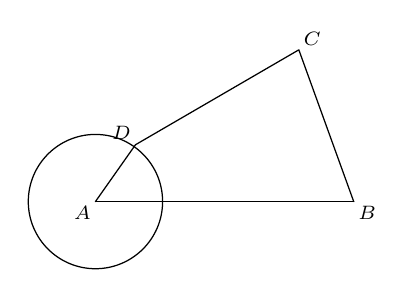
\begin{tikzpicture}[
  x=0.82cm,y=0.82cm,line width=0.45pt,line cap=round,line join=round,
  every node/.style={font=\scriptsize,inner sep=1.5pt}
]
  \coordinate (A) at (0,0);
  \coordinate (B) at (4,0);
  \coordinate (D) at (0.62,0.88);
  \coordinate (C) at (3.15,2.35);

  % The source shows a complete circle centered visually at A; it is not labelled as a trajectory.
  \draw (A) circle[radius=1.04];
  \draw (A)--(B);
  \draw (A)--(D)--(C)--(B);

  \node[below left] at (A) {$A$};
  \node[below right] at (B) {$B$};
  \node[above right] at (C) {$C$};
  \node[above left] at (D) {$D$};
\end{tikzpicture}
\end{center}
\nopagebreak[4]
\begin{itemize}
\item (A) \(\left[\dfrac{5}{16},\dfrac{53}{80}\right]\)
\item (B) \(\left[\dfrac{5}{16},\dfrac{73}{80}\right]\)
\item (C) \(\left[\dfrac{5}{12},\dfrac{53}{80}\right]\)
\item (D) \(\left[\dfrac{5}{12},\dfrac{73}{80}\right]\)
\end{itemize}

\end{question}
\gkpart{二、填空题}

\begin{question}
\gkti{11}\textbf{（源 PDF 第2页）} 

已知直线 \(ax+y=0\) 与圆 \((x-2)^2+(y-2)^2=4\) 相切，则 \(a=\underline{\qquad}\)。

\end{question}
\begin{question}
\gkti{12}\textbf{（源 PDF 第2页）} 

已知等差数列 \(\{a_n\}\) 的前 \(n\) 项和为 \(S_n\)，且 \(S_6=6a_6+30\)，则公差 \(d=\underline{\qquad}\)，若 \(S_n\leq S_5\) 恒成立，则符合条件的 \(a_1\) 的一个取值为\(\underline{\qquad}\)。

\end{question}
\begin{question}
\gkti{13}\textbf{（源 PDF 第2页）} 

\begin{gktip}
【编者待核注】固定回忆版候选 PDF 上限为 \(3\lg 2\)（含等号）；第三方 PDF 作严格小于。固定来源字面照录，端点异文未裁定。
\end{gktip}

音高 \(y\)（单位:mel）与频率 \(f\)（单位：Hz）满足 \(y=\lg\left(1+\dfrac{f}{700}\right)\)，若 \(\lg 2\leq y\leq 3\lg 2\)，则 \(f\) 的取值范围为\(\underline{\qquad}\)。

\Needspace{0.4\textheight}
\end{question}
\begin{question}
\gkti{14}\textbf{（源 PDF 第2页）} 

已知三棱锥 \(A-BCD\)，\(AD=AB=AC=2\sqrt{2}\)，\(BD=BC=2\)，\(DC=2\sqrt{3}\)，则它的底面 \(BCD\) 的面积为\(\underline{\qquad}\)，体积为\(\underline{\qquad}\)。
\nopagebreak[4]
\begin{center}% Generator: hand-authored TikZ schematic traced from the fixed source-visible tetrahedron edges; projection is illustrative.
% Source ID: src-96ac0e772a0483bbf7cf803b94b1a1d8d8e1d2ae16b936b196e6abc05d1251ee
% PDF SHA-256: 7e840dc5c259cf05138337178794a58b6593dc7f2bf0d693826489856da416e9
% PDF page 2; question 14.
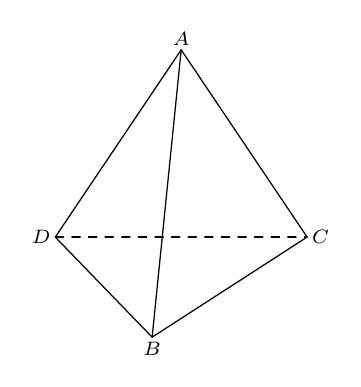
\begin{tikzpicture}[
  x=0.82cm,y=0.82cm,line width=0.45pt,line cap=round,line join=round,
  every node/.style={font=\scriptsize,inner sep=1.5pt}
]
  \coordinate (A) at (0,2.9);
  \coordinate (D) at (-1.95,0);
  \coordinate (C) at (1.95,0);
  \coordinate (B) at (-0.45,-1.55);

  % DC is the only hidden edge in the source.
  \draw[dashed] (D)--(C);
  \draw (A)--(D)--(B)--(C)--(A);
  \draw (A)--(B);

  \node[above] at (A) {$A$};
  \node[left] at (D) {$D$};
  \node[right] at (C) {$C$};
  \node[below] at (B) {$B$};
\end{tikzpicture}
\end{center}
\nopagebreak[4]
\end{question}
\begin{question}
\gkti{15}\textbf{（源 PDF 第2页）} 

\begin{gktip}
【编者待核注】固定回忆版候选 PDF 将“\(c=1\)”列为②、“\(c=0\)”列为③；第三方 PDF 交换这两个序号。两版来源链均不足以认证正式卷字面。
\end{gktip}

已知 \(f(x)=\lvert x^2-\cos x-c^2\rvert\)，给出下列四个结论：

① \(f(x)\) 在 \((-1,1]\) 上有最小值和最大值；

② \(c=1,\ x\in(-1,2]\) 时，\(f(x)\) 有最大值；

③ \(c=0,\ f(x)=1\) 有3个解；

④ \(c>0,\ f(x)\) 与 \(y=c\) 有4个交点。

其中正确结论的序号是\(\underline{\qquad}\)。

\end{question}
\gkpart{三、解答题}

\begin{question}
\gkti{16}\textbf{（源 PDF 第2页）} 

已知函数 \(f(x)=2\sin\omega x\cos\varphi+2\cos\omega x\sin\varphi\)，\(\omega>0,\ \lvert\varphi\rvert<\dfrac{\pi}{2}\)。\(f(x)\) 最小正周期为 \(\pi\)，且 \(f(0)>0,\ f\left(\dfrac{\pi}{4}\right)=1\)。

(1) 求 \(\omega\text{、}\varphi\) 的值；

(2) 求 \(f(x)\) 的单调递减区间。

\end{question}
\begin{question}
\gkti{17}\textbf{（源 PDF 第3页）} 

现从全校学生中随机抽取200人统计数学成绩，成绩分组及对应人数如下：

\begin{center}
\begin{tabular}{lrrrrr}
\toprule
成绩分组 & \([81,94)\) & \([94,107)\) & \([107,120)\) & \([120,135)\) & \([135,150]\) \\
\midrule
人数 & 40 & 60 & 60 & 32 & 8 \\
\bottomrule
\end{tabular}
\end{center}

以频率估计概率，完成下列问题：

(1) 求数学成绩低于120分的概率；

(2) 从学校随机抽取4人，求2人不低于120且2人小于94的概率；

(3) 每组数据取左端、中间、右端，比较 \(s_{\text{左}}^2\text{、}s_{\text{中}}^2\text{、}s_{\text{右}}^2\) 的大小关系。

\Needspace{0.4\textheight}
\end{question}
\begin{question}
\gkti{18}\textbf{（源 PDF 第3页）} 

已知直三棱柱 \(ABC-A_1B_1C_1\)，\(\angle BAC=90^\circ\)，\(AB=AC=2\)，\(BB_1=\sqrt{2}\)，\(E\text{、}D\) 分别为 \(A_1B_1\text{、}AC\) 的中点。
\nopagebreak[4]
\begin{center}% Generator: hand-authored TikZ schematic traced from the fixed source-visible prism edges and auxiliary lines; projection is illustrative.
% Source ID: src-96ac0e772a0483bbf7cf803b94b1a1d8d8e1d2ae16b936b196e6abc05d1251ee
% PDF SHA-256: 7e840dc5c259cf05138337178794a58b6593dc7f2bf0d693826489856da416e9
% PDF page 3; question 18.
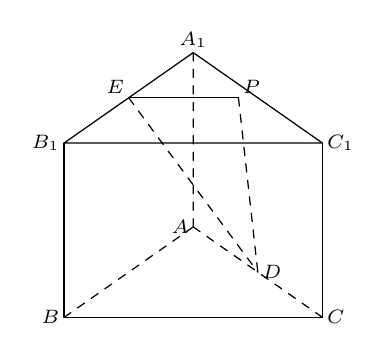
\begin{tikzpicture}[
  x=0.82cm,y=0.82cm,line width=0.45pt,line cap=round,line join=round,
  every node/.style={font=\scriptsize,inner sep=1.5pt}
]
  \coordinate (A)  at (0,-0.2);
  \coordinate (B)  at (-2,-1.6);
  \coordinate (C)  at (2,-1.6);
  \coordinate (A1) at (0,2.5);
  \coordinate (B1) at (-2,1.1);
  \coordinate (C1) at (2,1.1);
  \coordinate (E)  at (-1,1.8);
  \coordinate (D)  at (1,-0.9);
  \coordinate (P)  at (0.7,1.8);

  % Hidden prism edges from the source.
  \draw[dashed] (A)--(B) (A)--(C) (A)--(A1);

  % Auxiliary lines: EP is solid; ED and PD are dashed in the source.
  \draw[dashed] (E)--(D) (P)--(D);
  \draw (E)--(P);

  % Visible prism edges.
  \draw (B)--(C) (B)--(B1) (C)--(C1);
  \draw (A1)--(B1)--(C1)--cycle;

  \node[above] at (A1) {$A_1$};
  \node[left] at (B1) {$B_1$};
  \node[right] at (C1) {$C_1$};
  \node[left] at (B) {$B$};
  \node[right] at (C) {$C$};
  \node[left] at (A) {$A$};
  \node[above left] at (E) {$E$};
  \node[above right] at (P) {$P$};
  \node[right] at (D) {$D$};
\end{tikzpicture}
\end{center}
\nopagebreak[4]
(1) 证明：\(DE\parallel\)平面 \(BB_1C_1C\)；

(2) 点 \(P\) 在平面 \(A_1B_1C_1\) 内，且 \(EP\parallel B_1C_1\)，再从条件①、条件②、条件③这三个条件中选择一个作为已知，使得 \(P\) 唯一确定，求平面 \(PAD\) 与平面 \(PDE\) 的夹角的余弦值。

① \(PA=PD\)；

② \(PA\perp BC\)；

③ \(BB_1\parallel\)平面 \(PDE\)。

注：如果选择条件①、条件②、条件③分别解答，按第一个解答计分。

\end{question}
\begin{question}
\gkti{19}\textbf{（源 PDF 第4页）} 

已知椭圆 \(E:\dfrac{x^2}{a^2}+\dfrac{y^2}{b^2}=1\ (a>b>0)\) 的一个顶点是 \((2,0)\)，离心率为 \(\dfrac{1}{2}\)。

(1) 求 \(E\) 的方程；

(2) 过点 \(A(1,1)\)，斜率为 \(k\ (k\ne\pm1)\) 的直线交椭圆 \(E\) 于 \(B\text{、}C\) 两点，\(B\) 关于 \(y=x\) 的对称点为 \(D\)，\(DC\) 交 \(y=x\) 于 \(Q\)，若 \(\left\lvert S_{\triangle ABQ}-S_{\triangle ACQ}\right\rvert=\dfrac{5}{8}\)，求 \(k\)。

\end{question}
\begin{question}
\gkti{20}\textbf{（源 PDF 第4页）} 

设函数 \(f(x)=x^2+mx-4e^{nx-1}\ (n\in\mathbb{Z})\)，曲线 \(y=f(x)\) 在点 \((-1,f(-1))\) 处的切线方程为 \(4x+e^2y+e^2+8=0\)。

(1) 求 \(m\text{，}n\) 的值；

(2) 求 \(f(x)\) 的极值点个数；

(3) 求 \(y=kx-1\ (k>0)\) 与 \(f(x)\) 交点个数。

\end{question}
\begin{question}
\gkti{21}\textbf{（源 PDF 第5页）} 

设 \(A=(a_{ij})_{m\times n}\) 是一个 \(m\) 行 \(n\) 列的数阵，且数阵中的每一项 \(a_{ij}\in\{-1,1\}\)，都等于1或$-$1。若对任意 \(1\leq i,p\leq m,\ 1\leq j,q\leq n\)，其中 \(i\ne p,\ j\ne q\)，且 \(\bigl\lvert\lvert i-p\rvert-\lvert j-q\rvert\bigr\rvert=2\)，都有 \(a_{ij}+a_{iq}+a_{pj}+a_{pq}=0\)，则称数阵 \(A\) 具有性质 \(P\)。

\Needspace{5\baselineskip}
(1) 判断下列两个数表是否具有性质 \(P\)。

\nopagebreak[4]
\[
A_1=
\begin{pmatrix}
1&1&-1&1\\
-1&1&-1&1
\end{pmatrix},
\qquad
A_2=
\begin{pmatrix}
1&1&-1&-1\\
1&-1&1&-1\\
-1&1&-1&1
\end{pmatrix}.
\]

(2) 若 \(m=5,\ n=4\)，则具有性质 \(P\) 的数阵 \(A\) 中1的个数最多是多少？

(3) 若 \(m=n=6,\ a_{11}=1\)，且数阵 \(A\) 具有性质 \(P\)，证明：对任意 \(i\text{，}j\in\{1,2,3,4,5,6\}\)，都有 \(a_{ij}=a_{i1}a_{1j}\)。

\end{question}
\clearpage
\pdfbookmark[1]{参考答案与详细解析}{sec:s}
\Needspace{8\baselineskip}
\begin{center}{\Large\bfseries 参考答案与详细解析}\end{center}
\medskip
% answers.tex —— 2026 年·北京卷数学（回忆版，内部候选） · 参考答案与详细解析片段
% 由 tools/generate_projects.py 依来源总账自 2026/2026_数学真题_北京回忆版_试题.md + 2026/2026_数学真题_北京回忆版_解析正文.md + 2026/2026_数学真题_北京回忆版_答案要点.md 生成，勿手改（改源 MD 后重跑）


\begin{gktip}
固定候选 PDF 仅含题面；以下解析为本库独立推导，非原卷解析或官方答案。Q10、Q13 的候选来源异文尚未裁定；Q18 条件③不能唯一确定点，均保留阻塞标记。
\end{gktip}

\gkpart{一、单选题}

\begin{answer}
\gksolhead{1}{}

\textbf{题目}（源 PDF 第1页）：

已知集合 \(M=\{x\mid -1<x<3\}\)，\(N=\{x\mid x\geq 2\}\)，则 \(M\cup N=\)（　）

\begin{itemize}
\item (A) \((2,3)\)
\item (B) \((-1,+\infty)\)
\item (C) \([2,3)\)
\item (D) \((-1,2]\)
\end{itemize}

\Needspace{4\baselineskip}
\textbf{解析}

\(M=(-1,3)\)，\(N=[2,+\infty)\)，故并集为 \((-1,+\infty)\)，选 B。

\gkanswer{答案：B}

\end{answer}
\begin{answer}
\gksolhead{2}{}

\textbf{题目}（源 PDF 第1页）：

已知 \(z_1=3-2i\)，\(z_2=-1+4i\)，则 \(\lvert z_1+z_2\rvert=\)（　）

\begin{itemize}
\item (A) \(2\sqrt{2}\)
\item (B) \(i\)
\item (C) \(2\)
\item (D) \(8\)
\end{itemize}

\Needspace{4\baselineskip}
\textbf{解析}

\(z_1+z_2=2+2i\)，所以 \(|z_1+z_2|=\sqrt{2^2+2^2}=2\sqrt2\)，选 A。

\gkanswer{答案：A，\(2\sqrt2\)}

\end{answer}
\begin{answer}
\gksolhead{3}{}

\textbf{题目}（源 PDF 第1页）：

已知双曲线 \(C:\dfrac{x^2}{a^2}-\dfrac{y^2}{4}=1\ (a>0)\) 的渐近线方程为 \(y=\pm\dfrac{2}{3}x\)，则 \(a\) 的值为（　）

\begin{itemize}
\item (A) \(2\)
\item (B) \(3\)
\item (C) \(4\)
\item (D) \(9\)
\end{itemize}

\Needspace{4\baselineskip}
\textbf{解析}

双曲线的渐近线斜率为 \(\pm\dfrac{2}{a}\)。由 \(\dfrac2a=\dfrac23\) 得 \(a=3\)，选 B。

\gkanswer{答案：B，\(a=3\)}

\end{answer}
\begin{answer}
\gksolhead{4}{}

\textbf{题目}（源 PDF 第1页）：

已知 \((a-\sqrt{x})^7\) 的展开式中的 \(x^2\) 的系数是 \(280\)，则 \(a=\)（　）

\begin{itemize}
\item (A) \(2\)
\item (B) \(-2\)
\item (C) \(1\)
\item (D) \(-1\)
\end{itemize}

\Needspace{4\baselineskip}
\textbf{解析}

\Needspace{5\baselineskip}
\((a-\sqrt{x})^7\) 中 \(x^2\) 项取四个 \(-\sqrt{x}\) 因子，系数为
\nopagebreak[4]
\[
\binom74a^3=35a^3=280.
\]
因此 \(a=2\)，选 A。

\gkanswer{答案：A，\(a=2\)}

\end{answer}
\begin{answer}
\gksolhead{5}{}

\textbf{题目}（源 PDF 第1页）：

下列函数 \(f(x)\) 是奇函数且在定义域上单调递增的是（　）

\begin{itemize}
\item (A) \(f(x)=\dfrac{1}{x^2+1}\)
\item (B) \(f(x)=\sin x\)
\item (C) \(f(x)=2^{-x}-2^x\)
\item (D) \(f(x)=\ln\dfrac{5+x}{5-x}\)
\end{itemize}

\Needspace{4\baselineskip}
\textbf{解析}

\Needspace{5\baselineskip}
只有 D 在定义域 \((-5,5)\) 上同时为奇函数且严格递增：
\nopagebreak[4]
\[
f(-x)=-f(x),\qquad f'(x)=\frac{10}{25-x^2}>0.
\]
故选 D。

\gkanswer{答案：D}

\end{answer}
\begin{answer}
\gksolhead{6}{}

\textbf{题目}（源 PDF 第1页）：

已知向量 \(\vec a,\ \vec b\) 满足 \(\lvert\vec a-\vec b\rvert=2\)，\(\vec a=(2,0)\)，则 \(\lvert\vec b\rvert\) 的最大值为（　）

\begin{itemize}
\item (A) \(1\)
\item (B) \(2\)
\item (C) \(3\)
\item (D) \(4\)
\end{itemize}

\Needspace{4\baselineskip}
\textbf{解析}

\(|\vec a-\vec b|=2\) 表示 \(\vec b\) 位于以 \(\vec a=(2,0)\) 为圆心、半径2的圆上。由三角不等式 \(|\vec b|\le|\vec a|+2=4\)，沿正 \(x\) 方向可取到等号，选 D。

\gkanswer{答案：D，最大值 \(4\)}

\end{answer}
\begin{answer}
\gksolhead{7}{}

\textbf{题目}（源 PDF 第1页）：

\(\{a_n\}\)，\(\{b_n\}\) 是无穷数列，则“存在常数 \(M\)，使 \(a_n\leq M\leq b_n\ (n=1,2,3,\cdots)\)”是“\(a_n\leq b_n\ (n=1,2,3,\cdots)\)”的（　）

\begin{itemize}
\item (A) 充分不必要条件
\item (B) 必要不充分条件
\item (C) 充分必要条件
\item (D) 既不充分也不必要条件
\end{itemize}

\Needspace{4\baselineskip}
\textbf{解析}

若有常数 \(M\) 满足对所有 \(n\)，\(a_n\le M\le b_n\)，则必有 \(a_n\le b_n\)，所以前者是后者的充分条件。反向不成立，例如 \(a_n=n,b_n=n+1\) 逐项满足 \(a_n\le b_n\)，却不存在大于等于所有 \(a_n\) 的有限常数 \(M\)。选 A。

\gkanswer{答案：A，充分不必要条件}

\end{answer}
\begin{answer}
\gksolhead{8}{}

\textbf{题目}（源 PDF 第1页）：

\(f(x)=\sin(x+\varphi)\ (0<\varphi<2\pi)\)，将 \(f(x)\) 向 \(x\) 轴正方向平移 \(3\varphi\) 个单位，得到的函数图像与 \(f(x)\) 图像关于 \(x\) 轴对称，则 \(\varphi\) 的取值个数为（　）

\begin{itemize}
\item (A) \(1\)
\item (B) \(2\)
\item (C) \(3\)
\item (D) \(4\)
\end{itemize}

\Needspace{4\baselineskip}
\textbf{解析}

\Needspace{5\baselineskip}
向右平移 \(3\varphi\) 后为 \(g(x)=\sin(x-2\varphi)\)。关于 \(x\) 轴对称要求
\nopagebreak[4]
\[
\sin(x-2\varphi)=-\sin(x+\varphi)\quad(\forall x),
\]
即 \(2\sin(x-\varphi/2)\cos(3\varphi/2)=0\) 对任意 \(x\) 成立。因此 \(\cos(3\varphi/2)=0\)，在 \(0<\varphi<2\pi\) 内有 \(\varphi=\pi/3,\pi,5\pi/3\)，共3个，选 C。

\gkanswer{答案：C，共 \(3\) 个值}

\end{answer}
\begin{answer}
\gksolhead{9}{}

\textbf{题目}（源 PDF 第1页）：

学校组织高一、高二学生参观甲、乙两地博物馆，每位学生可自主选择一处前往．已知高一学生总人数多于高二学生总人数，前往甲地的全体学生总数多于前往乙地的全体学生总数，则（　）

\begin{itemize}
\item (A) 去甲地的高一学生人数多于去乙地的高一学生人数
\item (B) 去甲地的高一学生人数多于去乙地的高二学生人数
\item (C) 去甲地的高一学生人数不多于去乙地的高二学生人数
\item (D) 去乙地的高二学生人数不少于去甲地的高二学生人数
\end{itemize}

\Needspace{4\baselineskip}
\textbf{解析}

\Needspace{5\baselineskip}
记去甲地的高一、高二人数分别为 \(x,y\)，去乙地的高一、高二人数分别为 \(z,w\)。题设给出
\nopagebreak[4]
\[
x+z>y+w,\qquad x+y>z+w.
\]
两式相加得 \(2x>2w\)，故 \(x>w\)，选 B。

\gkanswer{答案：B}

\end{answer}
\begin{answer}
\gksolhead{10}{}

\textbf{题目}（源 PDF 第1–2页）：

\begin{gktip}
【编者待核注】固定回忆版候选 PDF 的 Q10 选项忠实照录于下。第三方六页 PDF 的四个选项区间均有端点或区间异文；来源报告记录逐项差异，版本归属未核，不据此择定选项。
\end{gktip}

摇杆机械装置，如图，\(A\text{，}B\) 为定点，\(C\text{，}D\) 是动点，\(AD=1\text{，}CD=3\text{，}BC=\dfrac{5}{2}\text{，}AB=4\)，则 \(\cos\angle ABC\) 的取值范围（　）
\nopagebreak[4]
\begin{center}% Generator: hand-authored TikZ schematic traced from the fixed source-visible four-bar outline and circle; all proportions are illustrative.
% Source ID: src-96ac0e772a0483bbf7cf803b94b1a1d8d8e1d2ae16b936b196e6abc05d1251ee
% PDF SHA-256: 7e840dc5c259cf05138337178794a58b6593dc7f2bf0d693826489856da416e9
% PDF page 2; question 10.
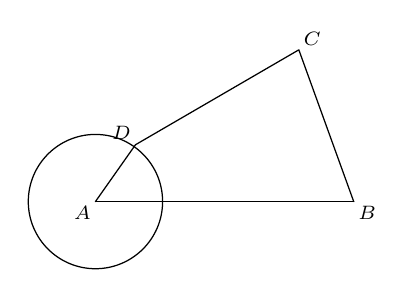
\begin{tikzpicture}[
  x=0.82cm,y=0.82cm,line width=0.45pt,line cap=round,line join=round,
  every node/.style={font=\scriptsize,inner sep=1.5pt}
]
  \coordinate (A) at (0,0);
  \coordinate (B) at (4,0);
  \coordinate (D) at (0.62,0.88);
  \coordinate (C) at (3.15,2.35);

  % The source shows a complete circle centered visually at A; it is not labelled as a trajectory.
  \draw (A) circle[radius=1.04];
  \draw (A)--(B);
  \draw (A)--(D)--(C)--(B);

  \node[below left] at (A) {$A$};
  \node[below right] at (B) {$B$};
  \node[above right] at (C) {$C$};
  \node[above left] at (D) {$D$};
\end{tikzpicture}
\end{center}
\nopagebreak[4]
\begin{itemize}
\item (A) \(\left[\dfrac{5}{16},\dfrac{53}{80}\right]\)
\item (B) \(\left[\dfrac{5}{16},\dfrac{73}{80}\right]\)
\item (C) \(\left[\dfrac{5}{12},\dfrac{53}{80}\right]\)
\item (D) \(\left[\dfrac{5}{12},\dfrac{73}{80}\right]\)
\end{itemize}

\Needspace{4\baselineskip}
\textbf{解析}

\Needspace{5\baselineskip}
按题图，\(D\) 是长度分别为 \(AD=1\)、\(DC=3\) 两杆的铰接点，故三角形 \(ADC\) 的三角不等式给出 \(2\le AC\le4\)，端点对应三点共线的极限位置。由余弦定理
\nopagebreak[4]
\[
\cos\angle ABC
=\frac{AB^2+BC^2-AC^2}{2AB\cdot BC}
=\frac{89/4-AC^2}{20}.
\]
该式随 \(AC\) 增大而减小；端点值分别为 \(73/80\) 与 \(5/16\)，所以固定回忆版候选题面的范围为 \([5/16,73/80]\)，对应其选项 B。第三方 PDF 的选项集合存在异文，版本未裁定，选项字母保留 U/PENDING。

\gkanswer{答案：U/PENDING；固定回忆版候选选项中 \(AC\in[5/16,73/80]\) 对应 B，异文未决}

\end{answer}
\gkpart{二、填空题}

\begin{answer}
\gksolhead{11}{}

\textbf{题目}（源 PDF 第2页）：

已知直线 \(ax+y=0\) 与圆 \((x-2)^2+(y-2)^2=4\) 相切，则 \(a=\underline{\qquad}\)。

\Needspace{4\baselineskip}
\textbf{解析}

\Needspace{5\baselineskip}
圆心为 \((2,2)\)，半径为2。直线 \(ax+y=0\) 与圆相切，故
\nopagebreak[4]
\[
\frac{|2a+2|}{\sqrt{a^2+1}}=2.
\]
平方并化简得 \(8a=0\)，所以 \(a=0\)。

\gkanswer{答案：\(0\)}

\end{answer}
\begin{answer}
\gksolhead{12}{}

\textbf{题目}（源 PDF 第2页）：

已知等差数列 \(\{a_n\}\) 的前 \(n\) 项和为 \(S_n\)，且 \(S_6=6a_6+30\)，则公差 \(d=\underline{\qquad}\)，若 \(S_n\leq S_5\) 恒成立，则符合条件的 \(a_1\) 的一个取值为\(\underline{\qquad}\)。

\Needspace{4\baselineskip}
\textbf{解析}

\nopagebreak[4]
\[
S_6=3(2a_1+5d),\qquad 6a_6+30=6(a_1+5d)+30.
\]
\Needspace{5\baselineskip}
联立得 \(d=-2\)。于是 \(S_n=n(a_1+1-n)\)，并且
\nopagebreak[4]
\[
S_n-S_5=(n-5)(a_1-n-4).
\]
对 \(n=1,2,3,4\)，要求 \(a_1\ge n+4\)，合并为 \(a_1\ge8\)；对 \(n\ge6\)，要求 \(a_1\le n+4\)，合并为 \(a_1\le10\)。故可行范围为 \([8,10]\)，任选例如 \(a_1=8\)。

\gkanswer{答案：\(d=-2\)；\(a_1\in[8,10]\)，例如 \(a_1=8\)}

\end{answer}
\begin{answer}
\gksolhead{13}{}

\textbf{题目}（源 PDF 第2页）：

\begin{gktip}
【编者待核注】固定回忆版候选 PDF 上限为 \(3\lg 2\)（含等号）；第三方 PDF 作严格小于。固定来源字面照录，端点异文未裁定。
\end{gktip}

音高 \(y\)（单位:mel）与频率 \(f\)（单位：Hz）满足 \(y=\lg\left(1+\dfrac{f}{700}\right)\)，若 \(\lg 2\leq y\leq 3\lg 2\)，则 \(f\) 的取值范围为\(\underline{\qquad}\)。

\Needspace{4\baselineskip}
\textbf{解析}

\Needspace{5\baselineskip}
对 \(y=\lg(1+f/700)\) 单调递增，题设等价于
\nopagebreak[4]
\[
2\le1+\frac f{700}\le8,
\]
按固定回忆版候选题面的非严格上界，\(700\le f\le4900\) Hz；按第三方 PDF 的严格上界，条件计算为 \(700\le f<4900\) Hz。两种端点字面尚未裁定，最终端点答案保留 U/PENDING。

\gkanswer{答案：U/PENDING；固定回忆版候选为 \([700,4900]\)，第三方异文对应 \([700,4900)\)}

\end{answer}
\begin{answer}
\gksolhead{14}{}

\textbf{题目}（源 PDF 第2页）：

已知三棱锥 \(A-BCD\)，\(AD=AB=AC=2\sqrt{2}\)，\(BD=BC=2\)，\(DC=2\sqrt{3}\)，则它的底面 \(BCD\) 的面积为\(\underline{\qquad}\)，体积为\(\underline{\qquad}\)。
\nopagebreak[4]
\begin{center}% Generator: hand-authored TikZ schematic traced from the fixed source-visible tetrahedron edges; projection is illustrative.
% Source ID: src-96ac0e772a0483bbf7cf803b94b1a1d8d8e1d2ae16b936b196e6abc05d1251ee
% PDF SHA-256: 7e840dc5c259cf05138337178794a58b6593dc7f2bf0d693826489856da416e9
% PDF page 2; question 14.
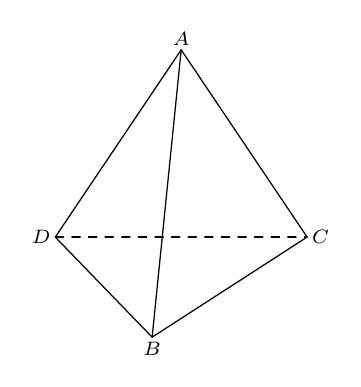
\begin{tikzpicture}[
  x=0.82cm,y=0.82cm,line width=0.45pt,line cap=round,line join=round,
  every node/.style={font=\scriptsize,inner sep=1.5pt}
]
  \coordinate (A) at (0,2.9);
  \coordinate (D) at (-1.95,0);
  \coordinate (C) at (1.95,0);
  \coordinate (B) at (-0.45,-1.55);

  % DC is the only hidden edge in the source.
  \draw[dashed] (D)--(C);
  \draw (A)--(D)--(B)--(C)--(A);
  \draw (A)--(B);

  \node[above] at (A) {$A$};
  \node[left] at (D) {$D$};
  \node[right] at (C) {$C$};
  \node[below] at (B) {$B$};
\end{tikzpicture}
\end{center}
\nopagebreak[4]
\Needspace{4\baselineskip}
\textbf{解析}

底面 \(BCD\) 是边长为2、2、\(2\sqrt3\) 的等腰三角形。以 \(DC\) 为底时，高为
\Needspace{5\baselineskip}
\(\sqrt{2^2-(\sqrt3)^2}=1\)，故底面积 \(S_{BCD}=\sqrt3\)。其外接圆半径
\nopagebreak[4]
\[
R=\frac{BD\cdot BC\cdot DC}{4S_{BCD}}=2.
\]
\Needspace{5\baselineskip}
由于 \(AB=AC=AD=2\sqrt2\)，顶点 \(A\) 在底面外接圆圆心的垂线上，棱锥高为 \(\sqrt{8-R^2}=2\)。体积为
\nopagebreak[4]
\[
V=\frac13S_{BCD}\cdot2=\frac{2\sqrt3}{3}.
\]

\gkanswer{答案：底面积 \(\sqrt3\)，体积 \(\dfrac{2\sqrt3}{3}\)}

\end{answer}
\begin{answer}
\gksolhead{15}{}

\textbf{题目}（源 PDF 第2页）：

\begin{gktip}
【编者待核注】固定回忆版候选 PDF 将“\(c=1\)”列为②、“\(c=0\)”列为③；第三方 PDF 交换这两个序号。两版来源链均不足以认证正式卷字面。
\end{gktip}

已知 \(f(x)=\lvert x^2-\cos x-c^2\rvert\)，给出下列四个结论：

① \(f(x)\) 在 \((-1,1]\) 上有最小值和最大值；

② \(c=1,\ x\in(-1,2]\) 时，\(f(x)\) 有最大值；

③ \(c=0,\ f(x)=1\) 有3个解；

④ \(c>0,\ f(x)\) 与 \(y=c\) 有4个交点。

其中正确结论的序号是\(\underline{\qquad}\)。

\Needspace{4\baselineskip}
\textbf{解析}

令 \(h(x)=x^2-\cos x\)，则 \(f(x)=|h(x)-c^2|\)。函数 \(h\) 为偶函数，且 \(h'(x)=2x+\sin x>0\)（\(x>0\)），最小值为 \(h(0)=-1\)。

\begin{itemize}
\item ①成立：\((-1,1]\) 上的函数值集合与 \([-1,1]\) 相同，因为 \(f\) 为偶函数，未取到的左端点值可由 \(x=1\) 取得；连续函数在对应紧区间上有最大、最小值。
\item ②成立：当 \(c=1\) 时，\(f(0)=2\)，而 \(f(2)=3-\cos2>2\)。连续函数在 \((-1,2]\) 的上确界不会因左端点缺失而丢失，因为 \(f(-1)=f(1)\) 且 \(1\) 在区间内，故最大值能取得。
\item ③成立：当 \(c=0\)，\(|h(x)|=1\) 等价于 \(h(x)=1\) 或 \(h(x)=-1\)。前者有两个对称解，后者仅在 \(x=0\) 取得，共3解。
\item ④成立：\(|h(x)-c^2|=c\) 等价于 \(h(x)=c^2+c\) 或 \(h(x)=c^2-c\)。对 \(c>0\)，两个水平值均大于 \(-1\)，且 \(h\) 偶、在正半轴严格递增，故每个水平各有两个解，共4个交点。
\end{itemize}

因此固定回忆版候选题面下正确序号为①②③④。第三方 PDF 只交换②、③的序号；在本题四项均成立的独立推导下，交换不改变该序号集合，但题面来源异文仍待核。

\gkanswer{答案：①②③④（②、③的原文序号有异文；两版下四项均成立）}

\end{answer}
\gkpart{三、解答题}

\begin{answer}
\gksolhead{16}{}

\textbf{题目}（源 PDF 第2页）：

已知函数 \(f(x)=2\sin\omega x\cos\varphi+2\cos\omega x\sin\varphi\)，\(\omega>0,\ \lvert\varphi\rvert<\dfrac{\pi}{2}\)。\(f(x)\) 最小正周期为 \(\pi\)，且 \(f(0)>0,\ f\left(\dfrac{\pi}{4}\right)=1\)。

(1) 求 \(\omega\text{、}\varphi\) 的值；

(2) 求 \(f(x)\) 的单调递减区间。

\Needspace{4\baselineskip}
\textbf{解析}

\gksubpart{(1) 求参数}

\Needspace{5\baselineskip}
由和角公式
\nopagebreak[4]
\[
f(x)=2\sin(\omega x+\varphi).
\]
\Needspace{5\baselineskip}
最小正周期为 \(\pi\)，故 \(2\pi/\omega=\pi\)，即 \(\omega=2\)。由 \(f(0)>0\)、\(|\varphi|<\pi/2\) 得 \(0<\varphi<\pi/2\)。再由
\nopagebreak[4]
\[
f(\pi/4)=2\sin(\pi/2+\varphi)=2\cos\varphi=1
\]
得 \(\varphi=\pi/3\)。

\gksubpart{(2) 单调区间}

\Needspace{5\baselineskip}
导数为 \(4\cos(2x+\pi/3)\)，函数在导数非正的最大区间上递减，因此
\nopagebreak[4]
\[
\left[\frac\pi{12}+k\pi,\frac{7\pi}{12}+k\pi\right],\quad k\in\mathbb Z.
\]
端点导数为0，但包含端点后函数仍在整个区间上严格递减。

\gkanswer{答案（1）：\(\omega=2,\ \varphi=\dfrac\pi3\)}

\gkanswer{答案（2）：\(\left[\dfrac\pi{12}+k\pi,\dfrac{7\pi}{12}+k\pi\right]\)，\(k\in\mathbb{Z}\)}

\end{answer}
\begin{answer}
\gksolhead{17}{}

\textbf{题目}（源 PDF 第3页）：

现从全校学生中随机抽取200人统计数学成绩，成绩分组及对应人数如下：

\begin{center}
\begin{tabular}{lrrrrr}
\toprule
成绩分组 & \([81,94)\) & \([94,107)\) & \([107,120)\) & \([120,135)\) & \([135,150]\) \\
\midrule
人数 & 40 & 60 & 60 & 32 & 8 \\
\bottomrule
\end{tabular}
\end{center}

以频率估计概率，完成下列问题：

(1) 求数学成绩低于120分的概率；

(2) 从学校随机抽取4人，求2人不低于120且2人小于94的概率；

(3) 每组数据取左端、中间、右端，比较 \(s_{\text{左}}^2\text{、}s_{\text{中}}^2\text{、}s_{\text{右}}^2\) 的大小关系。

\Needspace{4\baselineskip}
\textbf{解析}

五组频率依次为 \(0.2,0.3,0.3,0.16,0.04\)。

\gksubpart{(1) 低于120分的概率}

1. 低于120分的频率为 \((40+60+60)/200=0.8\)。
\gksubpart{(2) 指定抽取事件概率}

\Needspace{5\baselineskip}
2. 不低于120分与低于94分的单人概率估计均为 \(0.2\)。按频率估计所用的独立多项分布模型，恰有两人属于每一类的概率为
\nopagebreak[4]
\[
   \frac{4!}{2!2!}(0.2)^2(0.2)^2=\frac6{625}.
\]
   该答案依赖上述模型解释；若题目意指从已抽样的200人中无放回抽取，概率模型不同，原题未明确这种有限总体解释。
\gksubpart{(3) 方差比较}

\Needspace{5\baselineskip}
3. 左端、中点、右端代表值分别为 \((81,94,107,120,135)\)、\((87.5,100.5,113.5,127.5,142.5)\)、\((94,107,120,135,150)\)。按组频率计算的均值分别为 \(101.1,107.8,114.5\)，方差分别为 \(209.49,218.41,227.65\)（以总频数200为分母）。除以199的样本方差具有相同顺序，故
\nopagebreak[4]
\[
   s_{\text{左}}^2<s_{\text{中}}^2<s_{\text{右}}^2.
\]

\gkanswer{答案（1）：\(0.8\)}

\gkanswer{答案（2）：独立多项分布模型下 \(\dfrac6{625}\)}

\gkanswer{答案（3）：\(s_{\text{左}}^2<s_{\text{中}}^2<s_{\text{右}}^2\)}

\end{answer}
\begin{answer}
\gksolhead{18}{}

\textbf{题目}（源 PDF 第3页）：

已知直三棱柱 \(ABC-A_1B_1C_1\)，\(\angle BAC=90^\circ\)，\(AB=AC=2\)，\(BB_1=\sqrt{2}\)，\(E\text{、}D\) 分别为 \(A_1B_1\text{、}AC\) 的中点。
\nopagebreak[4]
\begin{center}% Generator: hand-authored TikZ schematic traced from the fixed source-visible prism edges and auxiliary lines; projection is illustrative.
% Source ID: src-96ac0e772a0483bbf7cf803b94b1a1d8d8e1d2ae16b936b196e6abc05d1251ee
% PDF SHA-256: 7e840dc5c259cf05138337178794a58b6593dc7f2bf0d693826489856da416e9
% PDF page 3; question 18.
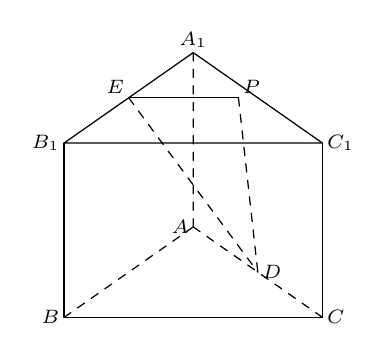
\begin{tikzpicture}[
  x=0.82cm,y=0.82cm,line width=0.45pt,line cap=round,line join=round,
  every node/.style={font=\scriptsize,inner sep=1.5pt}
]
  \coordinate (A)  at (0,-0.2);
  \coordinate (B)  at (-2,-1.6);
  \coordinate (C)  at (2,-1.6);
  \coordinate (A1) at (0,2.5);
  \coordinate (B1) at (-2,1.1);
  \coordinate (C1) at (2,1.1);
  \coordinate (E)  at (-1,1.8);
  \coordinate (D)  at (1,-0.9);
  \coordinate (P)  at (0.7,1.8);

  % Hidden prism edges from the source.
  \draw[dashed] (A)--(B) (A)--(C) (A)--(A1);

  % Auxiliary lines: EP is solid; ED and PD are dashed in the source.
  \draw[dashed] (E)--(D) (P)--(D);
  \draw (E)--(P);

  % Visible prism edges.
  \draw (B)--(C) (B)--(B1) (C)--(C1);
  \draw (A1)--(B1)--(C1)--cycle;

  \node[above] at (A1) {$A_1$};
  \node[left] at (B1) {$B_1$};
  \node[right] at (C1) {$C_1$};
  \node[left] at (B) {$B$};
  \node[right] at (C) {$C$};
  \node[left] at (A) {$A$};
  \node[above left] at (E) {$E$};
  \node[above right] at (P) {$P$};
  \node[right] at (D) {$D$};
\end{tikzpicture}
\end{center}
\nopagebreak[4]
(1) 证明：\(DE\parallel\)平面 \(BB_1C_1C\)；

(2) 点 \(P\) 在平面 \(A_1B_1C_1\) 内，且 \(EP\parallel B_1C_1\)，再从条件①、条件②、条件③这三个条件中选择一个作为已知，使得 \(P\) 唯一确定，求平面 \(PAD\) 与平面 \(PDE\) 的夹角的余弦值。

① \(PA=PD\)；

② \(PA\perp BC\)；

③ \(BB_1\parallel\)平面 \(PDE\)。

注：如果选择条件①、条件②、条件③分别解答，按第一个解答计分。

\Needspace{4\baselineskip}
\textbf{解析}

\gksubpart{(1) 证明线面平行}

\Needspace{5\baselineskip}
设
\nopagebreak[4]
\[
A=(0,0,0),\ B=(2,0,0),\ C=(0,2,0),\\
A_1=(0,0,\sqrt2),\ B_1=(2,0,\sqrt2),\ C_1=(0,2,\sqrt2).
\]
则 \(E=(1,0,\sqrt2)\)、\(D=(0,1,0)\)。侧面 \(BB_1C_1C\) 的法向量为 \((1,1,0)\)，而 \(\overrightarrow{DE}=(1,-1,\sqrt2)\) 与它垂直，故 \(DE\parallel\) 该平面。

\gksubpart{(2) 选择条件并计算夹角}

\Needspace{5\baselineskip}
由 \(EP\parallel B_1C_1\)，可设
\nopagebreak[4]
\[
P=(1-t,t,\sqrt2),\quad t\in\mathbb R.
\]
\Needspace{5\baselineskip}
选择条件①时，
\nopagebreak[4]
\[
PA^2=3-2t+2t^2,\qquad PD^2=4-4t+2t^2,
\]
\Needspace{5\baselineskip}
故 \(PA=PD\) 给出 \(t=1/2\)，唯一。条件②时，\(\overrightarrow{AP}\cdot\overrightarrow{BC}=0\) 给出
\nopagebreak[4]
\[
(1-t,t,\sqrt2)\cdot(-2,2,0)=4t-2=0,
\]
也得到唯一值 \(t=1/2\)。

条件③对任意 \(t\ne0\) 都成立：由 \(D,E,P\) 求出的平面法向量平行于 \((1,1,0)\)，所以竖直方向 \(BB_1\) 平行于该平面；\(t=0\) 时 \(P=E\)，三点不确定平面。因此③不能唯一确定 \(P\)。

\Needspace{5\baselineskip}
取①或②得到同一点 \(P=(1/2,1/2,\sqrt2)\)。此时平面 \(PDE\) 的法向量可取 \((1,1,0)\)，平面 \(PAD\) 的法向量可取 \((\sqrt2,0,-1/2)\)。所以两平面的夹角余弦为
\nopagebreak[4]
\[
\frac{|(1,1,0)\cdot(\sqrt2,0,-1/2)|}{\sqrt2\cdot(3/2)}=\frac23.
\]

\gkanswer{答案（1）：见解析版}

\gkanswer{答案（2）：U/PENDING；若取条件①或②，夹角余弦均为 \(\dfrac23\)；条件③不能唯一确定 \(P\)。}

\end{answer}
\begin{answer}
\gksolhead{19}{}

\textbf{题目}（源 PDF 第4页）：

已知椭圆 \(E:\dfrac{x^2}{a^2}+\dfrac{y^2}{b^2}=1\ (a>b>0)\) 的一个顶点是 \((2,0)\)，离心率为 \(\dfrac{1}{2}\)。

(1) 求 \(E\) 的方程；

(2) 过点 \(A(1,1)\)，斜率为 \(k\ (k\ne\pm1)\) 的直线交椭圆 \(E\) 于 \(B\text{、}C\) 两点，\(B\) 关于 \(y=x\) 的对称点为 \(D\)，\(DC\) 交 \(y=x\) 于 \(Q\)，若 \(\left\lvert S_{\triangle ABQ}-S_{\triangle ACQ}\right\rvert=\dfrac{5}{8}\)，求 \(k\)。

\Needspace{4\baselineskip}
\textbf{解析}

\gksubpart{(1) 求椭圆方程}

1. 顶点 \((2,0)\) 给出 \(a=2\)；离心率 \(c/a=1/2\)，故 \(c=1,b^2=a^2-c^2=3\)。椭圆方程为 \(x^2/4+y^2/3=1\)。
\gksubpart{(2) 求斜率}

\Needspace{5\baselineskip}
2. 设直线写作 \(y=kx+1-k\)，与椭圆交点的横坐标为 \(u,v\)，令 \(S=u+v,P=uv\)。代入椭圆并用韦达定理得
\nopagebreak[4]
\[
   S=\frac{8k(k-1)}{3+4k^2},\qquad P=\frac{4k^2-8k-8}{3+4k^2}.
\]
\Needspace{5\baselineskip}
   令 \(Q=(q,q)\)。将 \(B=(u,ku+1-k)\) 关于 \(y=x\) 对称得到 \(D=(ku+1-k,u)\)，由直线 \(DC\) 与 \(y=x\) 联立可得
\nopagebreak[4]
\[
   q-1=\frac{(u-1)(v-1)(k+1)}{S-2}=\frac{5(k+1)}{2(4k+3)}.
\]
\Needspace{5\baselineskip}
   椭圆内点 \(A=(1,1)\) 位于弦 \(BC\) 内部，故 \(u-1,v-1\) 异号，从而
\nopagebreak[4]
\[
   \bigl||u-1|-|v-1|\bigr|=|S-2|=\frac{2|4k+3|}{3+4k^2}.
\]
\Needspace{5\baselineskip}
   两个三角形以 \(AQ\) 为共同底边，结合面积的绝对值可得
\nopagebreak[4]
\[
   \left|S_{\triangle ABQ}-S_{\triangle ACQ}\right|
   =\frac12|1-k|\,|q-1|\,\bigl||u-1|-|v-1|\bigr|
   =\frac{5|1-k^2|}{2(3+4k^2)}.
\]
   令其等于 \(5/8\)。若 \(k^2\le1\)，得 \(k^2=1/8\)；若 \(k^2>1\)，方程无解。因此 \(k=\pm\sqrt2/4\)。当 \(k=-3/4\) 时 \(DC\parallel y=x\) 且不重合，交点 \(Q\) 不存在，须按题意排除；该值不在所得根中。

\gkanswer{答案（1）：\(\dfrac{x^2}{4}+\dfrac{y^2}{3}=1\)}

\gkanswer{答案（2）：\(k=\pm\dfrac{\sqrt2}{4}\)；\(k=-\dfrac34\) 时 \(Q\) 不存在。}

\end{answer}
\begin{answer}
\gksolhead{20}{}

\textbf{题目}（源 PDF 第4页）：

设函数 \(f(x)=x^2+mx-4e^{nx-1}\ (n\in\mathbb{Z})\)，曲线 \(y=f(x)\) 在点 \((-1,f(-1))\) 处的切线方程为 \(4x+e^2y+e^2+8=0\)。

(1) 求 \(m\text{，}n\) 的值；

(2) 求 \(f(x)\) 的极值点个数；

(3) 求 \(y=kx-1\ (k>0)\) 与 \(f(x)\) 交点个数。

\Needspace{4\baselineskip}
\textbf{解析}

\gksubpart{(1) 求参数}

\Needspace{5\baselineskip}
切线方程化为 \(y=-4x/e^2-1-8/e^2\)，故在 \(x=-1\) 处函数值为 \(-1-4/e^2\)，斜率为 \(-4/e^2\)。将这两项分别代入 \(f(-1)\) 与 \(f'(-1)\)，并消去 \(m\)，得到
\nopagebreak[4]
\[
(n+1)e^{-n-1}=2e^{-2}.
\]
因 \(n\in\mathbb Z\)，只有 \(n=1\) 满足，继而 \(m=2\)。

\gksubpart{(2) 求极值点个数}

此时 \(f'(x)=2x+2-4e^{x-1}\)，\(f''(x)=2-4e^{x-1}\)：\(f'\) 先严格递增后严格递减，且 \(f'(-\infty)<0\)、\(f'(0)=2-4/e>0\)、\(f'(1)=0\)，故有两个零点，函数有2个极值点。

\gksubpart{(3) 求交点个数}

\Needspace{5\baselineskip}
交点方程可写成
\nopagebreak[4]
\[
H(x)=kx,\qquad H(x)=(x+1)^2-4e^{x-1}.
\]
对 \(x\ge0\)，令 \(L(x)=\ln\dfrac{4e^{x-1}}{(x+1)^2}\)。其导数为 \((x-1)/(x+1)\)，故在 \(x=1\) 取最小值0，得到 \(H(x)\le0\)；而 \(kx>0\)（\(x>0\)），所以正半轴无交点，\(x=0\) 也不是交点。

\Needspace{5\baselineskip}
对 \(x<0\)，令 \(G(x)=H(x)/x\)。有
\nopagebreak[4]
\[
G'(x)=\frac{(x-1)(x+1-4e^{x-1})}{x^2}>0.
\]
这里第二因子在 \(x<0\) 为负：其最大值在 \(x=1-\ln4\) 取得，等于 \(1-\ln4<0\)。又 \(G(x)\to-\infty\)（\(x\to-\infty\)），\(G(x)\to+\infty\)（\(x\to0^-\)），所以方程 \(G(x)=k\) 对每个 \(k>0\) 恰有一个解。因此交点数为1。

\gkanswer{答案（1）：\(m=2,n=1\)}

\gkanswer{答案（2）：2 个极值点}

\gkanswer{答案（3）：1 个交点}

\end{answer}
\begin{answer}
\gksolhead{21}{}

\textbf{题目}（源 PDF 第5页）：

设 \(A=(a_{ij})_{m\times n}\) 是一个 \(m\) 行 \(n\) 列的数阵，且数阵中的每一项 \(a_{ij}\in\{-1,1\}\)，都等于1或$-$1。若对任意 \(1\leq i,p\leq m,\ 1\leq j,q\leq n\)，其中 \(i\ne p,\ j\ne q\)，且 \(\bigl\lvert\lvert i-p\rvert-\lvert j-q\rvert\bigr\rvert=2\)，都有 \(a_{ij}+a_{iq}+a_{pj}+a_{pq}=0\)，则称数阵 \(A\) 具有性质 \(P\)。

\Needspace{5\baselineskip}
(1) 判断下列两个数表是否具有性质 \(P\)。

\nopagebreak[4]
\[
A_1=
\begin{pmatrix}
1&1&-1&1\\
-1&1&-1&1
\end{pmatrix},
\qquad
A_2=
\begin{pmatrix}
1&1&-1&-1\\
1&-1&1&-1\\
-1&1&-1&1
\end{pmatrix}.
\]

(2) 若 \(m=5,\ n=4\)，则具有性质 \(P\) 的数阵 \(A\) 中1的个数最多是多少？

(3) 若 \(m=n=6,\ a_{11}=1\)，且数阵 \(A\) 具有性质 \(P\)，证明：对任意 \(i\text{，}j\in\{1,2,3,4,5,6\}\)，都有 \(a_{ij}=a_{i1}a_{1j}\)。

\Needspace{4\baselineskip}
\textbf{解析}

\gksubpart{(1) 判断两个数表}

1. \(A_1\) 中第1、4列构成的合法四格和为2，故不满足 \(P\)；\(A_2\) 仅有第1、2行与第2、3行分别配第1、4列的两格，和均为0，故满足 \(P\)。
\gksubpart{(2) 求 1 的最多个数}

2. 对第1、4行，令 \(t_j=a_{1j}+a_{4j}\)。约束给出 \(t_j+t_{j+1}=0\)，故 \((t_1,t_2,t_3,t_4)=(u,-u,u,-u)\)，两行共4个1；第2、5行同理，第三行至多4个1，总数至多12。以 \(+\) 表示1、\(-\) 表示$-$1，取五行为 \(\mathtt{+--+},\mathtt{-++-},\mathtt{++++},\mathtt{-++-},\mathtt{+--+}\) 的矩阵 \(A\)，它满足全部12个约束并含12个1，故上界可达。
\gksubpart{(3) 证明题设结论}

3. 精确有理数消元得到52条约束的秩为34，零空间基 \(U,V\) 见独立求解复核报告，故 \(A=\alpha U+\beta V\)。由 \(a_{11}=1\) 得 \(\beta=1\)，再由 \(a_{12}\in\{\pm1\}\) 得 \(\alpha=\pm1\)；\(\alpha=-1\) 会使 \(a_{33}=-3\)，与 \(a_{ij}\in\{\pm1\}\) 矛盾，故 \(\alpha=1\)。此时前三行均为 \((1,1,1,-1,-1,-1)\)，后三行为其相反数，从而 \(a_{ij}=a_{i1}a_{1j}\)。可复现的约束生成与消元代码见独立求解复核报告。

\gkanswer{答案（1）：\(A_1\) 否，\(A_2\) 是。}

\gkanswer{答案（2）：最多 12 个 1。}

\gkanswer{答案（3）：\(a_{ij}=a_{i1}a_{1j}\)。}

\end{answer}
\end{document}
